\section{Aim}

To Write a C/C++ POSIX compliant program to check the following limits:
\begin{enumerate}
	\item Number of clock ticks
	\item Maximum number of child processes
	\item Maximum path length
	\item Maximum number of characters in a file
	\item Maximum number of open files
\end{enumerate}

\section{Theory}

\subsection{sysconf - Get configuration information at runtime}

\subsubsection{Synopsis}

\begin{lstlisting}
#include <unistd.h>
long sysconf(int name);
\end{lstlisting}

\subsubsection{Description}

POSIX allows an application to test at compile or run time whether certain options are supported, or what the value is of certain configurable constants or limits. At compile time this is done by including <unistd.h> and/or <limits.h> and testing the value of certain macros.

At run time, one can ask for numerical values using the present function sysconf(). One can ask for numerical values that may depend on the file system a file is in using the calls fpathconf(3) and pathconf(3). One can ask for string values using confstr(3). The values obtained from these functions are system configuration constants. They do not change during the lifetime of a process.

\begin{description}
	\item clock ticks - \_SC\_CLK\_TCK \hfill \\
		The number of clock ticks per second.  The corresponding variable is obsolete.  It  was  of  course  called  CLK\_TCK.
	\item CHILD\_MAX - \_SC\_CHILD\_MAX \hfill \\
		The max number of simultaneous processes per user ID.  Must not be less than \_POSIX\_CHILD\_MAX (25).
	\item OPEN\_MAX - \_SC\_OPEN\_MAX \hfill \\
		The maximum number of files that a process can have open at any time.  Must not be less than \_POSIX\_OPEN\_MAX (20).
\end{description}

\subsection{fpathconf, pathconf - Get configuration values for files}

\subsubsection{Synopsis}

\begin{lstlisting}
#include <unistd.h>
long fpathconf(int fd, int name);
long pathconf(char *path, int name);
\end{lstlisting}

\subsubsection{Description}

fpathconf() gets a value for the configuration option name for the open file descriptor fd.

pathconf() gets a value for configuration option name for the filename path.

The corresponding macros defined in <unistd.h> are minimum values; if an application wants to take advantage of values which may change, a call to fpathconf() or pathconf() can be made, which may yield more liberal results.

\begin{description}
	\item \_PC\_PATH\_MAX \hfill \\
		returns the maximum length of a relative pathname when path or fd is the current working directory.  The  corresponding macro is \_POSIX\_PATH\_MAX.  
	\item \_PC\_NAME\_MAX \hfill \\
		returns the maximum length of a filename in the directory path or fd that the process is allowed to create.  The corresponding macro is \_POSIX\_NAME\_MAX.
\end{description}

\section{Code}

\begin{lstlisting}
#define _POSIX_SOURCE
#define _POSIX_C_SOURCE 199309L

#include "iostream"
#include <unistd.h>
using namespace std;

int main()
{
	cout << "No of clock ticks:" << sysconf(_SC_CLK_TCK) << endl;
	cout << "Maximum no of child processes:" << sysconf(_SC_CHILD_MAX) << endl;
	cout << "Maximum path length:" << pathconf("/",_PC_PATH_MAX) << endl;
	cout << "Maximum characters in a file name:" << pathconf("/",_PC_NAME_MAX) << endl;
	cout << "Maximum no of open files:" << sysconf(_SC_OPEN_MAX) << endl;
	return 0;
}
\end{lstlisting}

\section{Output}

%\emph{Commands for execution:-}

\begin{enumerate}
	\item Open a terminal.
	\item Change directory to the file location in the terminal.
	\item Run g++ usp01.c -o usp01.out in the terminal.
	\item If no errors, run ./usp01.out
\end{enumerate}

%\subsection{Screenshots:}\label{screenshots}

%\begin{figure}[htbp]
%\centering
%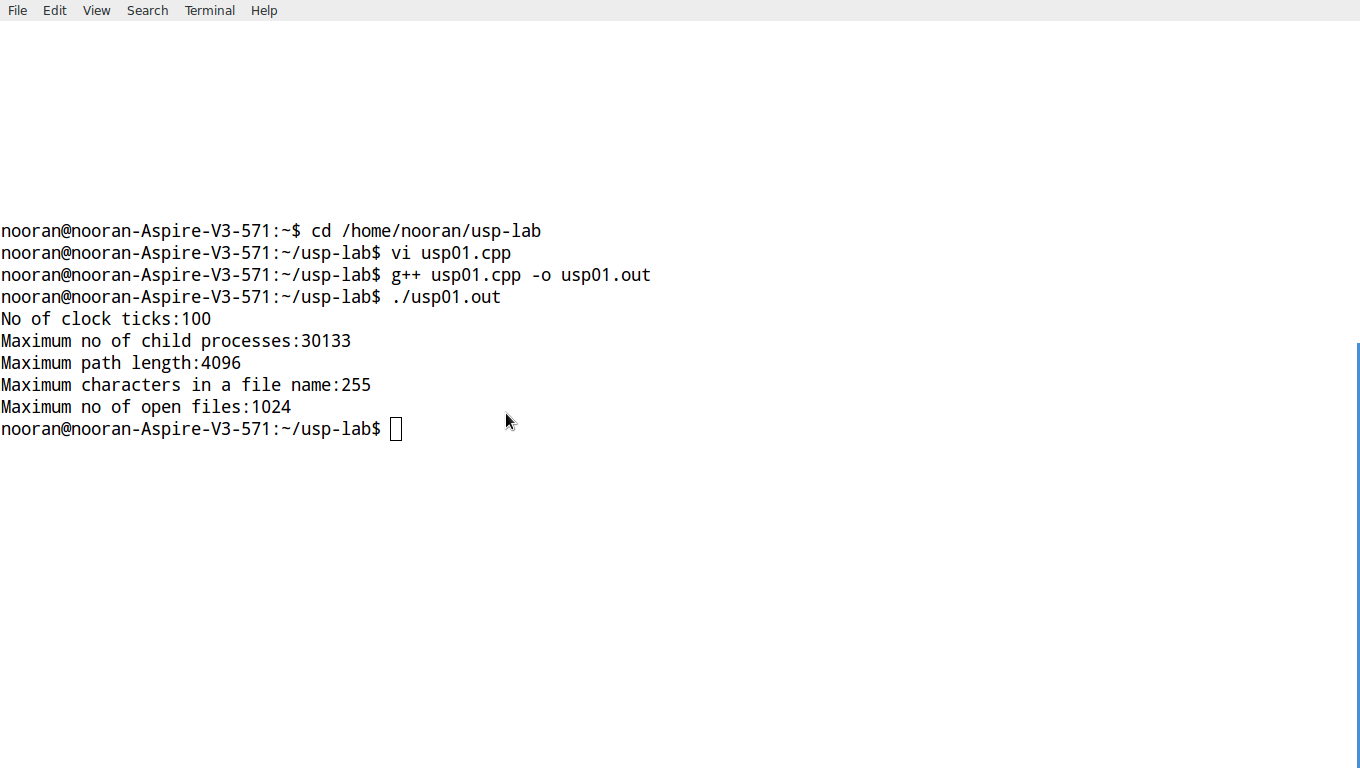
\includegraphics{usp-lab-01.png}
%\caption{not available}
%\end{figure}
